\documentclass[11pt,a4paper]{article}
\usepackage[margin=2.5cm]{geometry}
\usepackage{lmodern}
\usepackage[T1]{fontenc}
\usepackage{graphicx}
\usepackage{booktabs}
\usepackage{setspace}
\usepackage[hidelinks]{hyperref}
\setstretch{1.15}
\setlength{\parskip}{0.45em}
\setlength{\parindent}{0pt}

\begin{document}

{\LARGE News sentiment beyond the mean}

{\large What I plan to write up, and the results it will use}

Peter Prendergast \quad \textperiodcentered \quad 12 August 2026

\vspace{0.8em}
\hrule
\vspace{1em}

\section*{The question}

Most trading days a company turns up in more than one news story, and the standard approach is to score each story and take the average. My question is whether the average is the right summary: how should many same-day stories be rolled up into one firm-day sentiment signal, and does the shape of the day's scores tell you anything about the next day's return that the mean does not? My hypothesis is that it does, and that the useful part sits in the negative tail. There is a secondary question too: can a learned trade/no-trade threshold beat a fixed band on the same signal? Everything runs on one panel with one design --- nine aggregation rules against next-open returns, a chronological split, date-clustered inference, a multiple-testing correction fixed in advance, and explicit trading costs --- and the one rule that survives then gets translated into a portfolio.

I am choosing this question because it runs on the biggest and cleanest sample I have, because every experiment it needs is already done so I can start writing now, and because the answer has a proper shape to it: the mean fails, one distribution feature survives, trading it directly dies on costs, and using it to manage risk partly works. The other candidate questions are stuck waiting on publisher metadata or human labels that will not arrive before the deadline.

\section*{The data and the setup}

The panel comes from FNSPID news for 2011--2023: 715{,}546 firm-days with news across 570 priced US symbols and 3{,}262 trading sessions, scored with a pinned FinBERT checkpoint. Development ends in December 2019 and evaluation runs from January 2020. The nine rules are the natural ways to summarise a day's scores: mean hard label, mean and median continuous score, trimmed mean, negative-story share, score dispersion, strongest event, log-count weighted mean, and a decayed sentiment state. Each one is tested with daily cross-sectional rank correlations, HAC-adjusted $t$-statistics, and a Benjamini--Hochberg correction across the family. Portfolio results charge fixed costs with final liquidation --- 10 bps a side for the stock arms and 2 bps for the index-level volatility arms --- and strategy comparisons use five-session block bootstraps so clustered days do not flatter the precision.

\section*{The results I will use}

\textbf{Only one summary survives, and it is not the mean.} Across the nine rules, negative-story share is the only one that survives the correction (mean daily IC $-0.005433$, HAC $t = -3.119$); the mean-based rules cannot be told apart from zero (Figure~1). It still holds after dropping every firm-day within five sessions of an earnings event. Story type, publisher, and earnings-window conditioning all fail their corrections, and I report those nulls as results.

\begin{figure}[htbp]
\centering
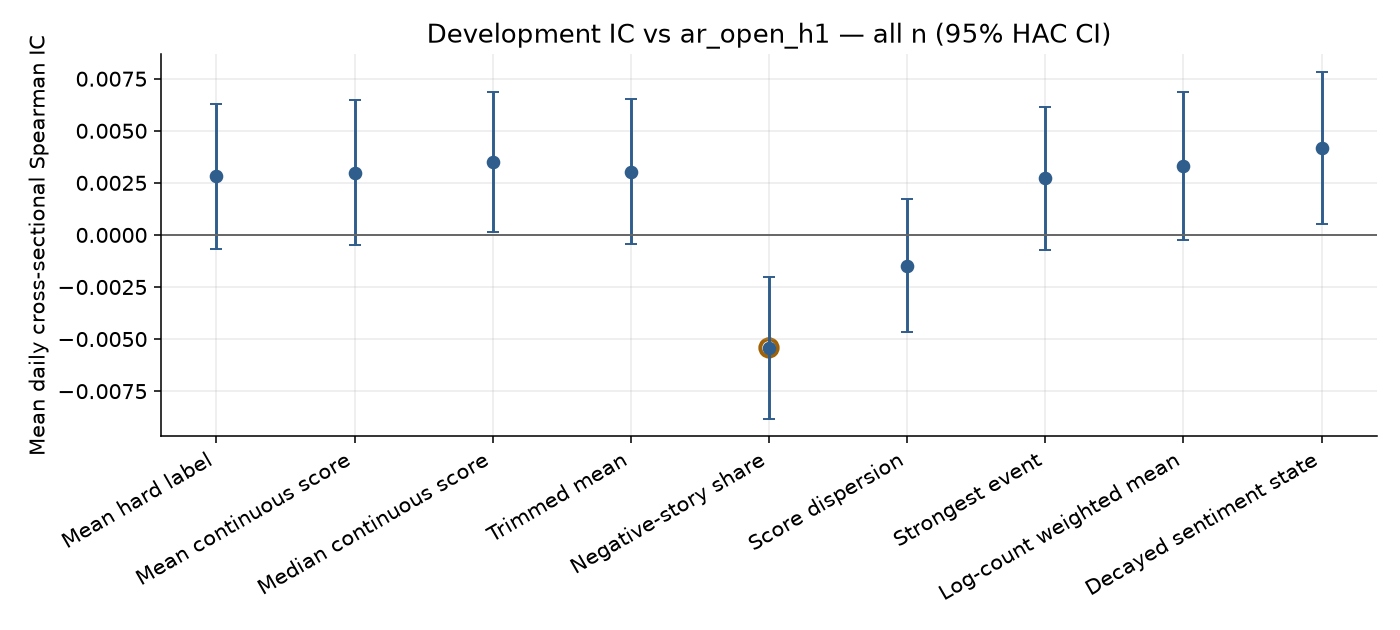
\includegraphics[width=\textwidth]{../../dissertation/figures/fig_aggregation_ic.png}
\caption{Daily rank correlation between each aggregation rule and the next-open abnormal return, development period, with 95\% HAC intervals. Negative-story share (circled) is the only rule that survives the correction.}
\end{figure}

\textbf{You cannot trade it directly.} Trading the signal daily turns the book over about 200 times a year, and the best break-even cost across the nine rules is 0.625 bps a side against the 10 bps I charge (Figure~2). Learned thresholds do not rescue it either: logistic, gradient-boosted, and MLP gates all sit at evaluation AUC around 0.50, and cash beats every learned policy. So the secondary question closes cleanly, and the gap between being able to detect the signal and being able to use it becomes a main theme of the write-up.

\begin{figure}[htbp]
\centering
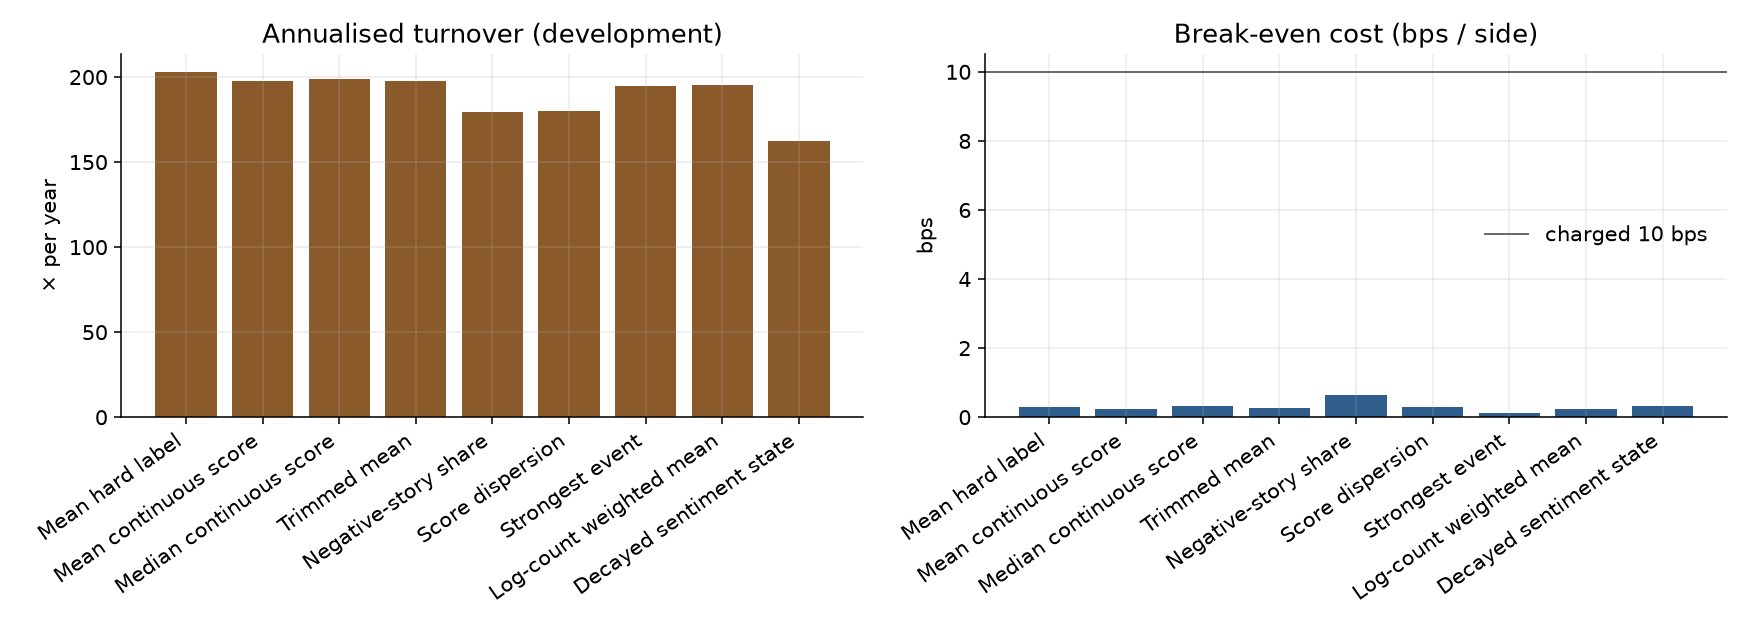
\includegraphics[width=\textwidth]{../../dissertation/figures/fig_turnover_breakeven.png}
\caption{Annualised turnover and break-even trading cost for each rule on the development block. The best break-even is 0.625 bps a side; the charged cost is 10 bps.}
\end{figure}

\textbf{It works as a risk dial.} The strongest standalone benchmark in the project is a sentiment-free HAR volatility target on SPY (evaluation net Sharpe 0.673, maximum drawdown $-15.73\%$, against 0.568 and $-32.05\%$ for buy-and-hold). Cutting that exposure when aggregate negative-story pressure is high lifts the net Sharpe to 0.835 and the total return from $+29.85\%$ to $+35.20\%$ at 2 bps a side (Figure~3), stays ahead at 10 bps, and the drop in downside-squared loss is statistically detectable ($p = 0.0148$). A walk-forward check on 2013--2019, fitted only on earlier data, finds the same thing: drawdown improves from $-12.53\%$ to $-8.57\%$ ($p = 0.0052$). The sentiment is timing risk, not return.

\begin{figure}[htbp]
\centering
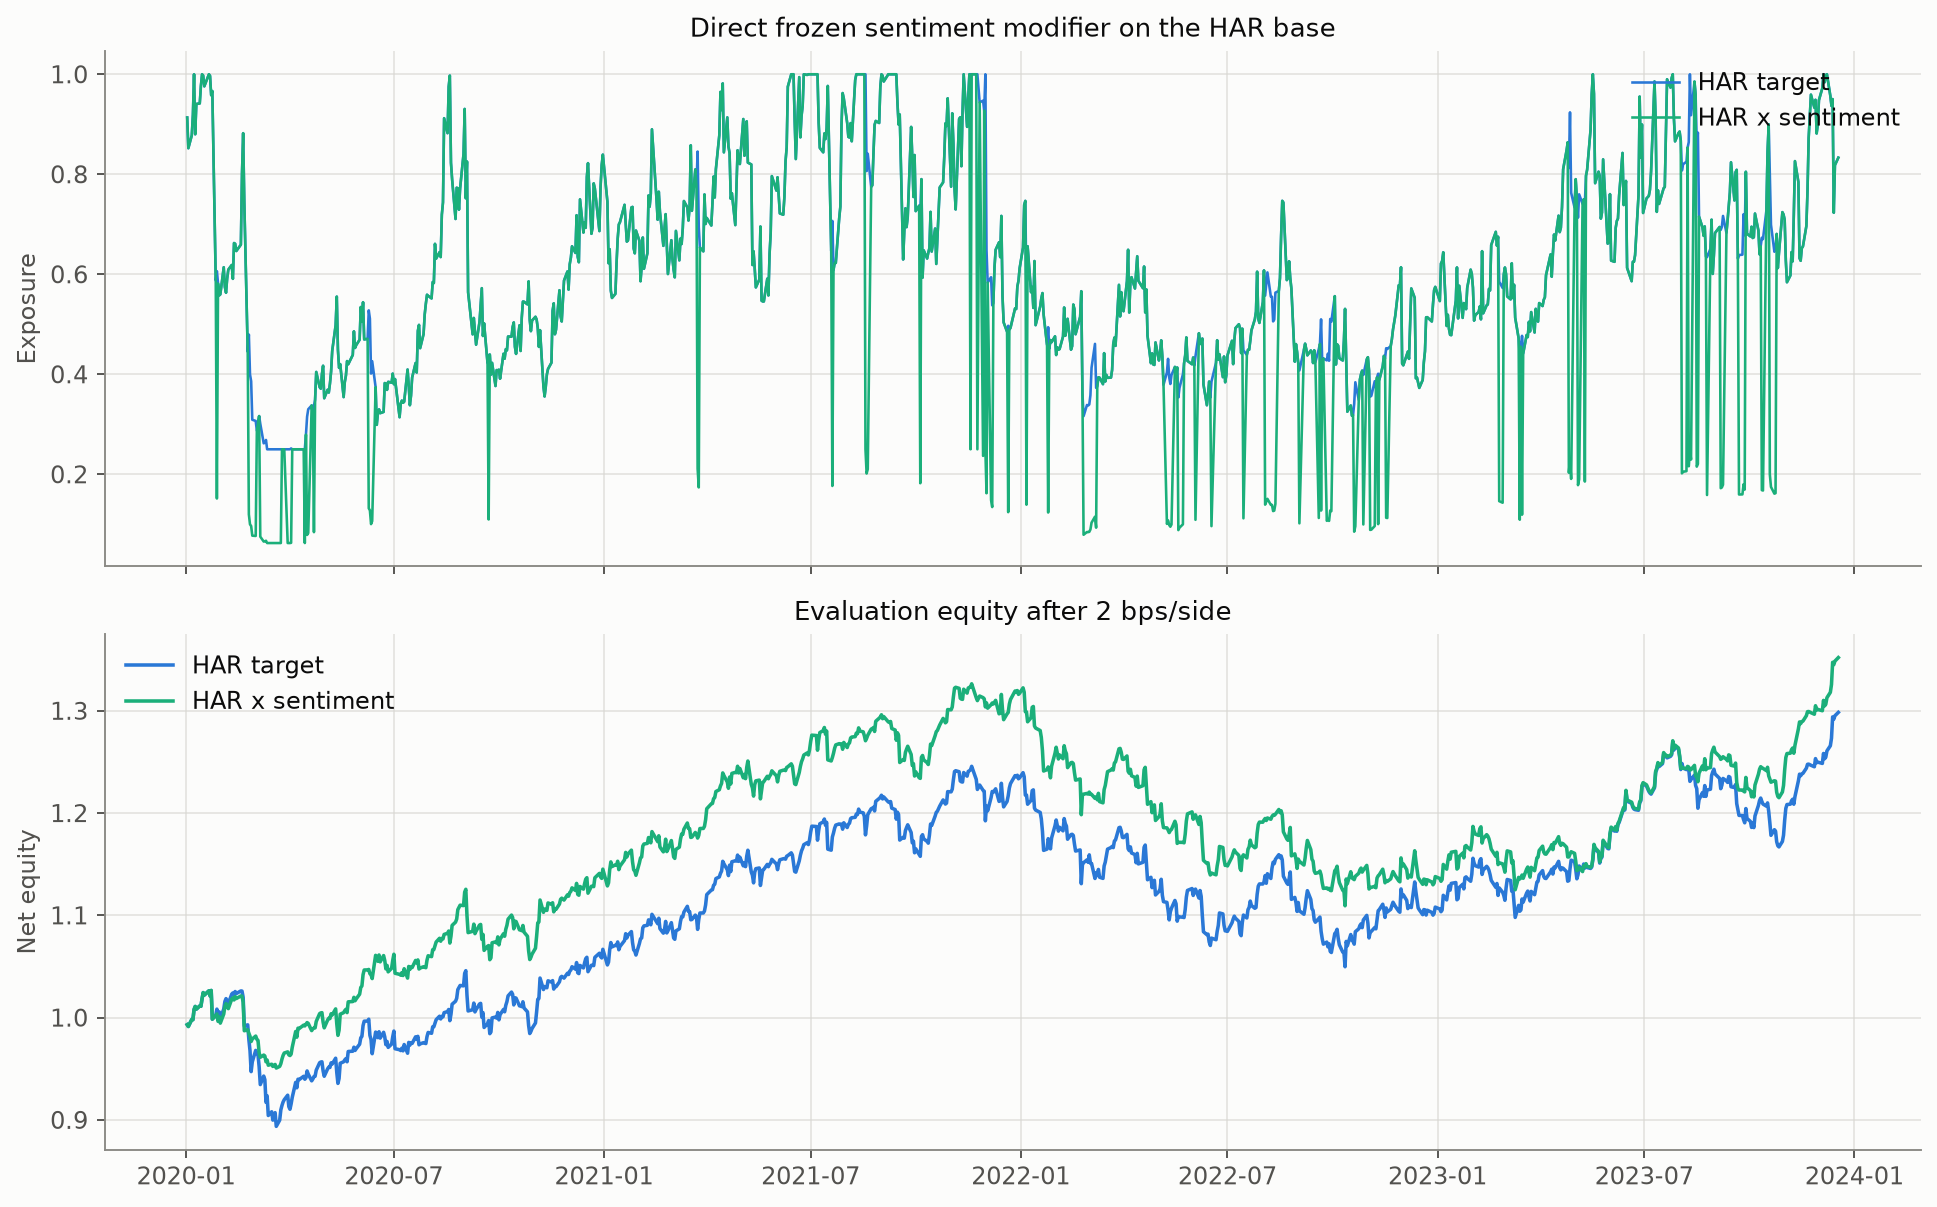
\includegraphics[width=\textwidth]{../../dissertation/figures/fig_har_sentiment_equity.png}
\caption{The HAR volatility target and the same target scaled down when aggregate negative-story pressure is high, evaluation period 2020--2023. The overlay changes exposure on a minority of days (top) and improves the net path (bottom).}
\end{figure}

\textbf{A placebo test backs the timing up.} I re-run the exact risk-off schedule at every possible circular shift of its dates. The observed timing beats 99.1\% of placements in 2020--2023 (exact $p = 0.0100$, BH $q = 0.0301$) and is suggestive but uncorrected in 2013--2019 (Figure~4). The claim is downside timing, strongest over 2020--2023.

\begin{figure}[htbp]
\centering
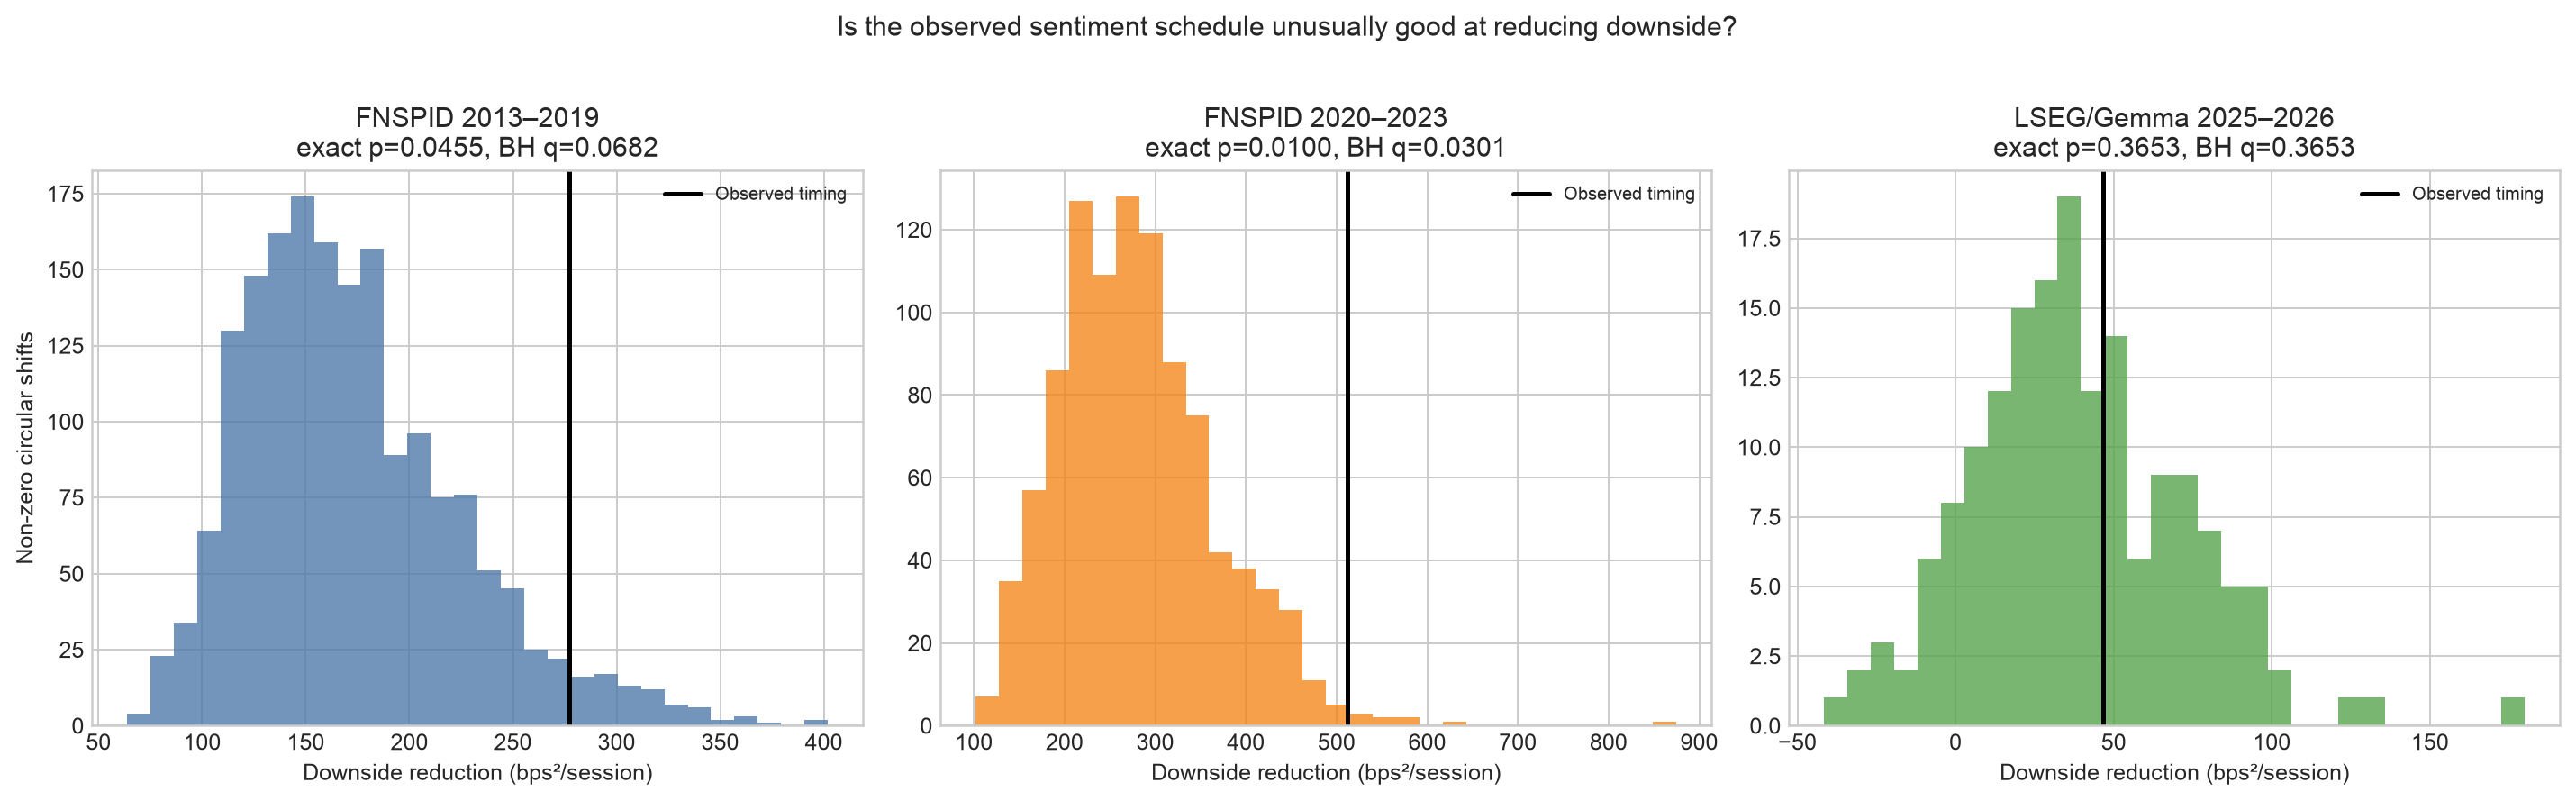
\includegraphics[width=\textwidth]{../../dissertation/figures/fig_downside_placebo.png}
\caption{Downside reduction of the observed sentiment schedule (vertical line) against every non-zero circular shift of the same schedule, in three separate regimes.}
\end{figure}

\textbf{A second data source keeps it honest.} A separate LSEG corpus (33 large caps plus a 22-name mid-cap arm, never pooled with FNSPID) gives the out-of-regime checks. The strongest strategy there earned a net Sharpe of 2.271 on the window it was picked on and $-0.354$ on an earlier block of the same names, even though headline-level scores were almost perfectly repeatable across model versions (rank correlation 0.989). Measuring sentiment consistently is not the same as having a signal that pays for its costs, and that contrast makes the main chapters stronger.

\section*{The shape of the write-up}

The write-up follows the UCL structure at about 10{,}000 words, with tables carrying the frozen numbers and the words carrying the interpretation. The registered replay on new LSEG dates (finishing December 2026 at the earliest) and the sealed materiality confirmation go in future directions as the specified confirmatory tests.

\begin{table}[htbp]
\centering
\begin{tabular}{lrl}
\toprule
Chapter & Words & Main sources \\
\midrule
1. Introduction & 1{,}000 & Research question, hypothesis, design summary \\
2. Literature review & 1{,}500 & Existing draft, extended to aggregation and costs \\
3. Methodology & 2{,}500 & Panel, split, scorer, nine rules, inference, cost model \\
4. Results & 3{,}500 & Aggregation family, thresholds, risk translation, robustness \\
5. Conclusions and future directions & 1{,}000 & Findings, limits, registered prospective test \\
\bottomrule
\end{tabular}
\caption{Planned chapter budget. Figures, tables, and equations sit outside the word count.}
\end{table}

The usual caveats --- a chronological rather than pristine split, machine labels still waiting on the human audit --- go in the limitations section, not the headline claims. Every number above is frozen in the repository with a manifest, and I am starting with the methodology and results chapters this week.

\end{document}
